\chapter{TypeDLT description}

The new TypeDLT (DayLightTing), written in the C++ programming language, performs the 3PM for dynamic, climate-based daylighting simulations of CFS taking in input the BSDF file.
The TypeDLT receives the following input from the weather file:
\begin{itemize}
\renewcommand{\labelitemi}{\tiny$\blacksquare$}
\item Latitude and longitude
\item Month, day of the month, hour of the day
\item Direct normal illuminance
\item Diffuse horizontal illuminance
\end{itemize}
In this way it can identify the building location (and thus calculate the sun path) and the information for the climate-based analysis. The following parameters are set in the Type's control panel:
\begin{itemize}
\renewcommand{\labelitemi}{\tiny$\blacksquare$}
\item Thermal zone for which the shading system is controlled
\item Shading state, determining which BSDF is used
\item Number of windows associated with the same shading state
\end{itemize}
These parameters are necessary to identify the thermal zone where CFS are controlled, which CFS assigned to that zone are controlled, and which are the initial conditions for the simulation. A BSDF data file has to be provided for each shading state. In order to independently control a series of thermal zones, the Type can be added as functional block to the simulation model multiple times, with different parameters, inputs, and outputs.
The outputs of the Type are:
\begin{itemize}
\renewcommand{\labelitemi}{\tiny$\blacksquare$}
\item Maximum (or average, minimum, etc.) illuminance value over the sensors grid
\item Current shading state
\end{itemize}
The control algorithm, defined through a series of equations which can involve inputs and outputs of other Types, the Type56, and the TypeDLT are interlinked. Loops between Types can be formed. By default, TRNSYS performs iterations after each time step until all parameters, inputs and outputs of every Type have converged. Therefore, the main difference with other integrated software is the time-step interaction of the TypeDLT with the other Types contained into the TRNSYS deck. \\
The control algorithm is not incorporated into the TypeDLT, but implemented through the "Equation" functional blocks that TRNSYS offers by default. This has the big advantage that the TypeDLT does not need to be recompiled every time the control strategy has changed and can thus be reused more easily by the user.
This approach gives the maximum flexibility in the setting of a shading control strategy, since it is possible to test custom control algorithm taking in account all the main aspects of a sustainable design: energy saving, thermal and visual comfort, but with the detriment of calculation time.

\begin{figure}[h]
\centering
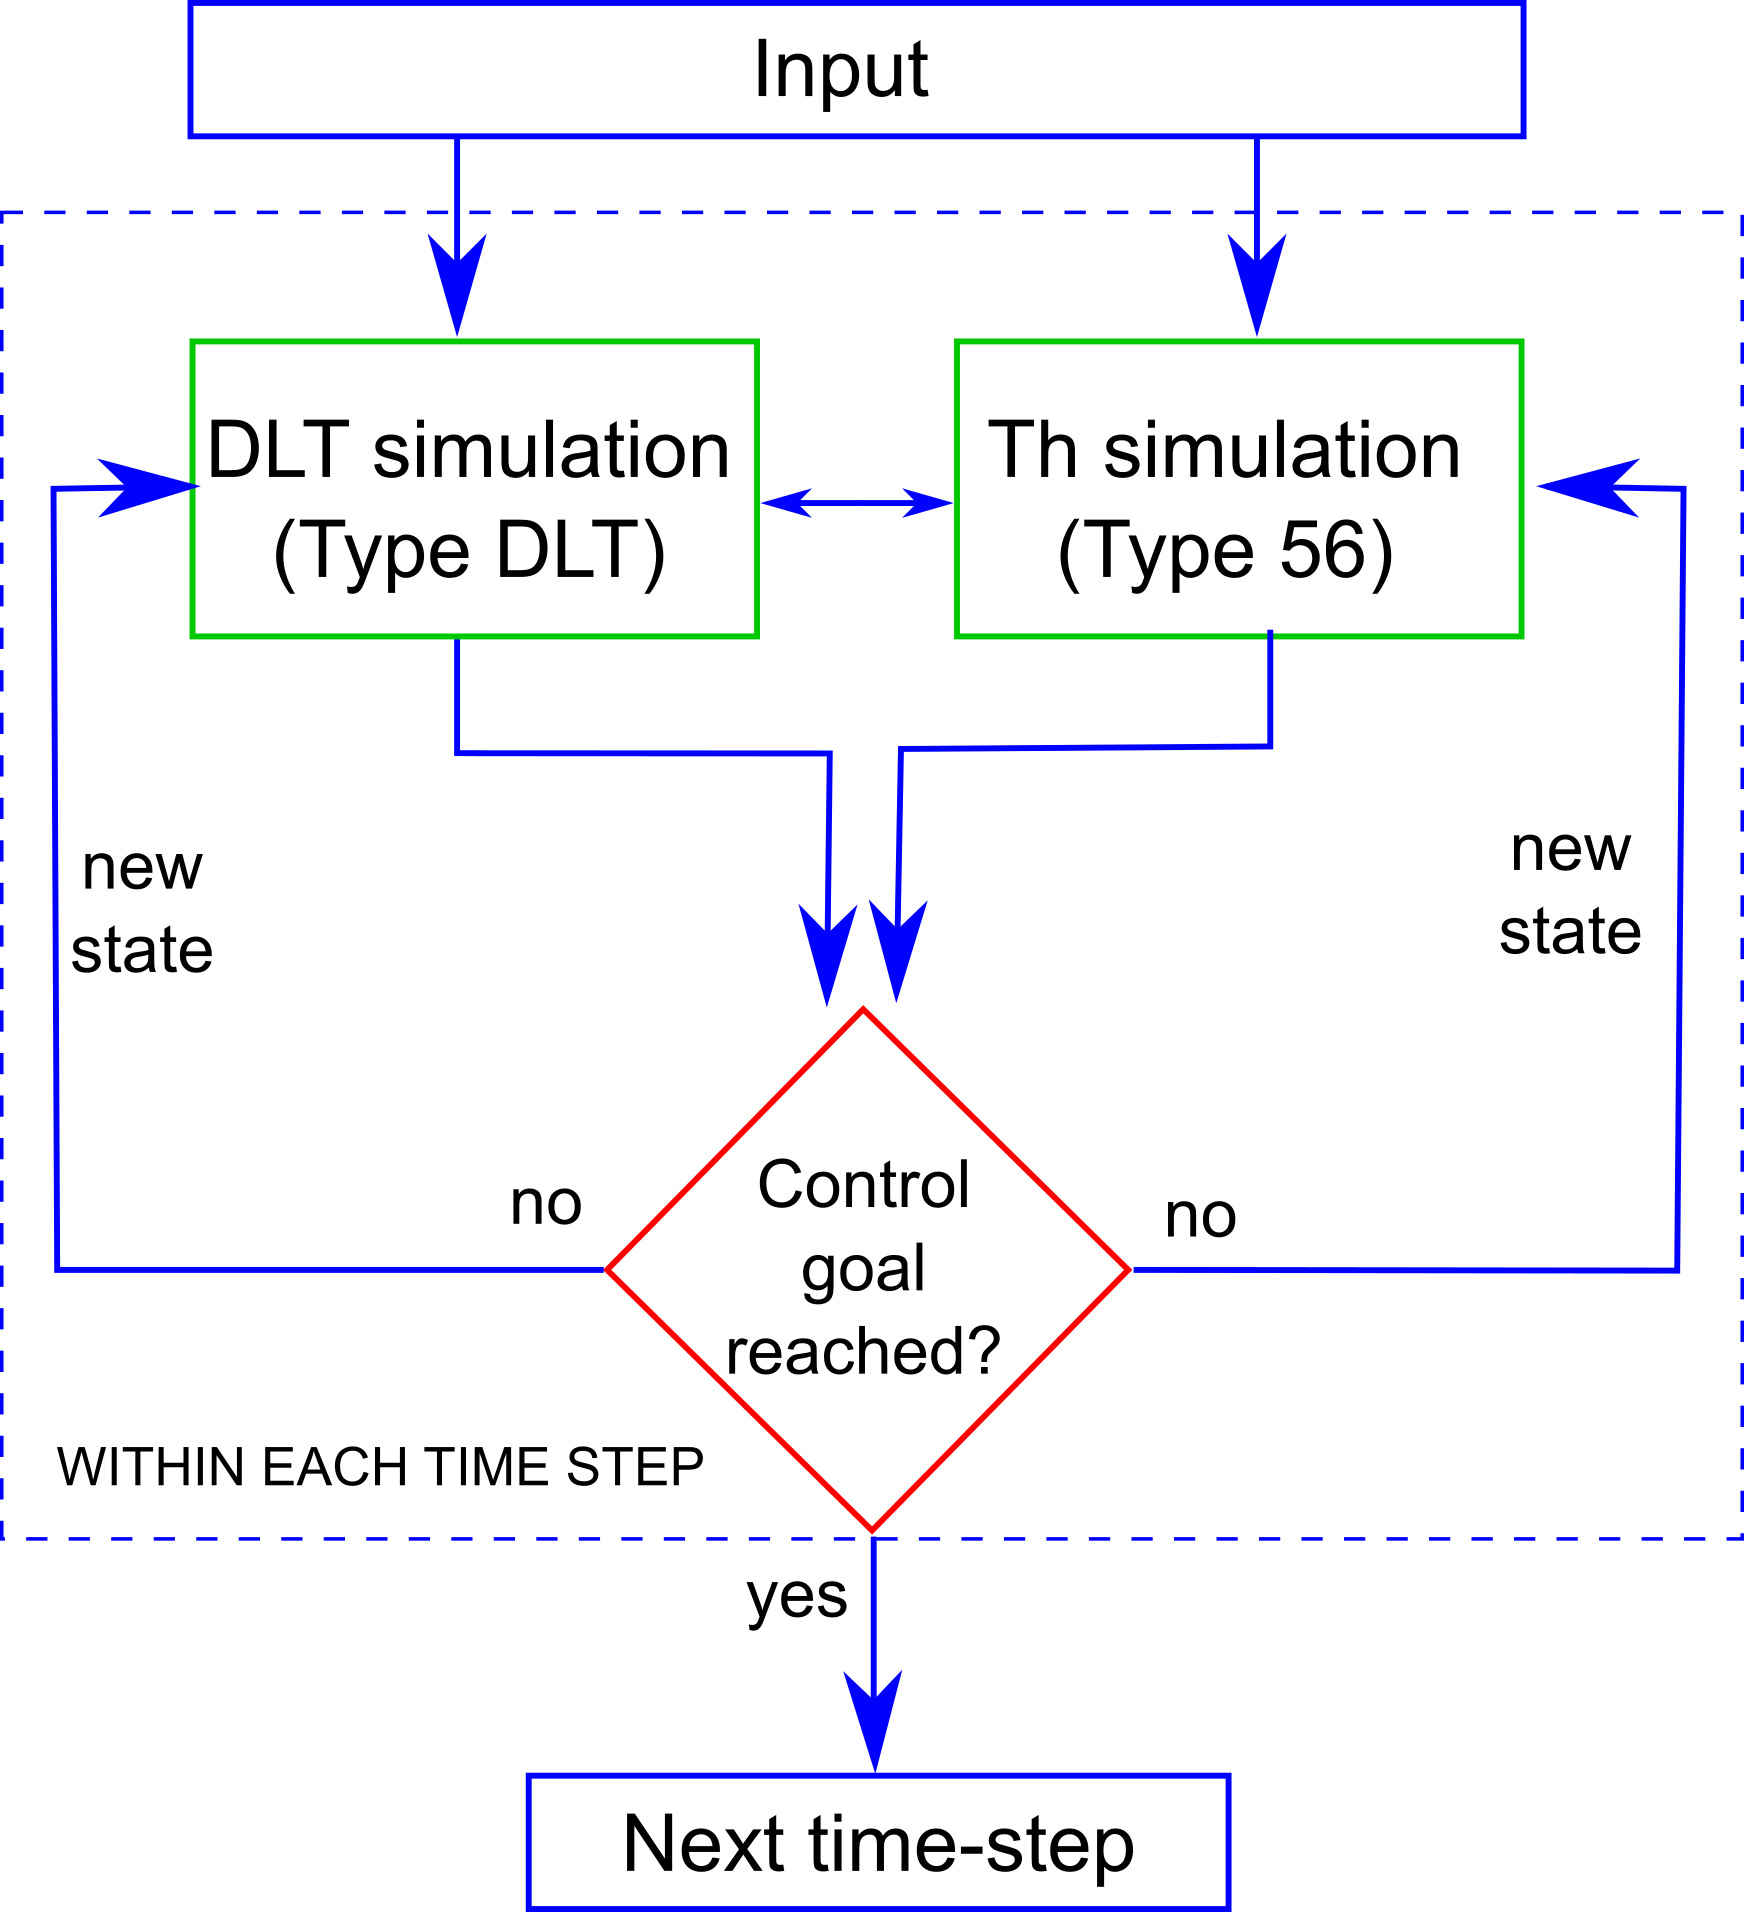
\includegraphics[width=0.7\textwidth]{control}
\caption{\label{img2:flow} Flow chart of the iteration process between daylighting and thermal simulation within each time step}
\end{figure}

Figure \ref{img2:flow} shows a typical workflow of the process. Both the daylighting (TypeDLT) and the thermal (Type56) simulations take their inputs. Then, the BSDF data and the Types' outputs are passed to a control "Equation" (a special functional block of TRNSYS in which an equation system can be defined) that modifies the shading states. By default, TRNSYS iterates until all Type outputs have reached convergence. Only then, it advances in time by performing the next time step.

%\begin{figure}[h]
%\centering
%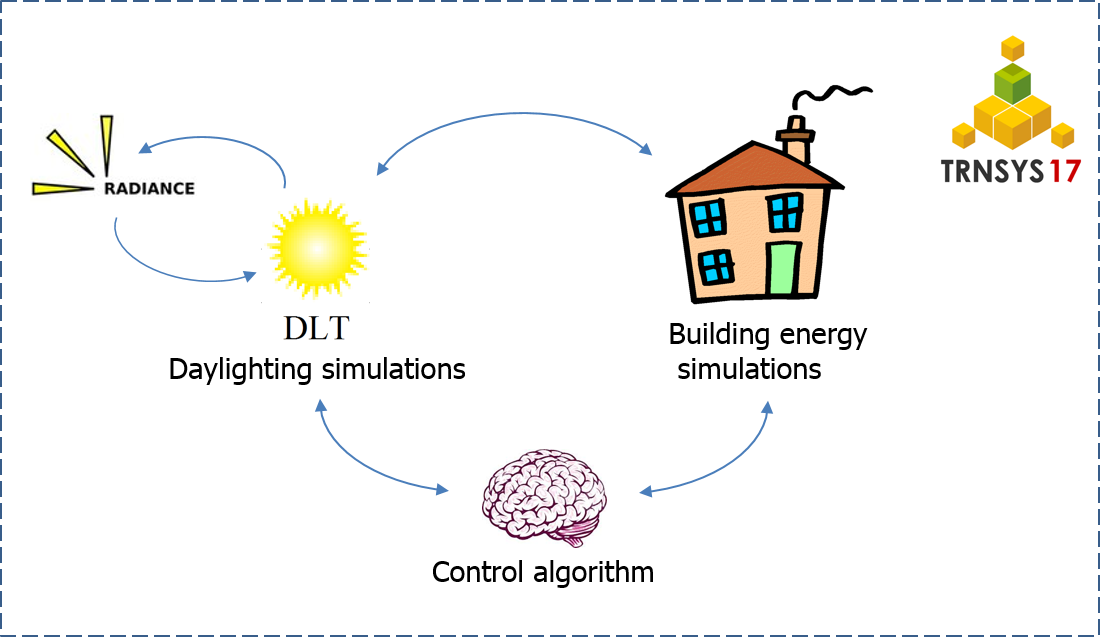
\includegraphics[width=0.9\textwidth]{deck}
%\caption{\label{img2:deck} Flow chart of the iteration process between daylighting and thermal simulation within each time step}
%\end{figure}
